\documentclass{beamer}

\usetheme{CambridgeUS}
\usecolortheme{dolphin}

\usepackage[spanish]{babel}
\usepackage[utf8]{inputenc}
\usepackage[T1]{fontenc}
\usepackage{pgfpages}
\usepackage{relsize}
\usepackage[style=authortitle]{biblatex}
\usepackage{epigraph}
\usepackage{caption}
\usepackage[labelformat=simple,subrefformat=simple]{subcaption}
\usepackage[capitalise, noabbrev]{cleveref}

\setbeameroption{show notes on second screen=right}

\setbeamertemplate{caption}{\raggedright\insertcaption\par}
\setbeamerfont{caption}{size=\scriptsize}
\setbeamertemplate{navigation symbols}{}

\captionsetup[figure]{labelformat=empty}

\graphicspath{{figures/}}

\addbibresource{sna.bib}
\addbibresource{presentation_sna.bib}

\renewcommand\thesubfigure{(\Alph{subfigure})}

\title[Inference of Socioeconomic Status]{Comparative Study of Methods for the Inference of Socioeconomic Status in a Communications Graph}
\subtitle{Presentación de Tesis}

\author{Martín~Fixman}

\date{Noviembre de 2018}

\institute[FCEN UBA]{Facultad de Ciencias Exactas y Naturales \\ Universidad de Buenos Aires}

\begin{document}

\begin{frame}
	\titlepage{} 
\end{frame}

\begin{frame}
	\tableofcontents{}
\end{frame}

\section{Introducción}

\begin{frame}

	\begin{figure}[b]
		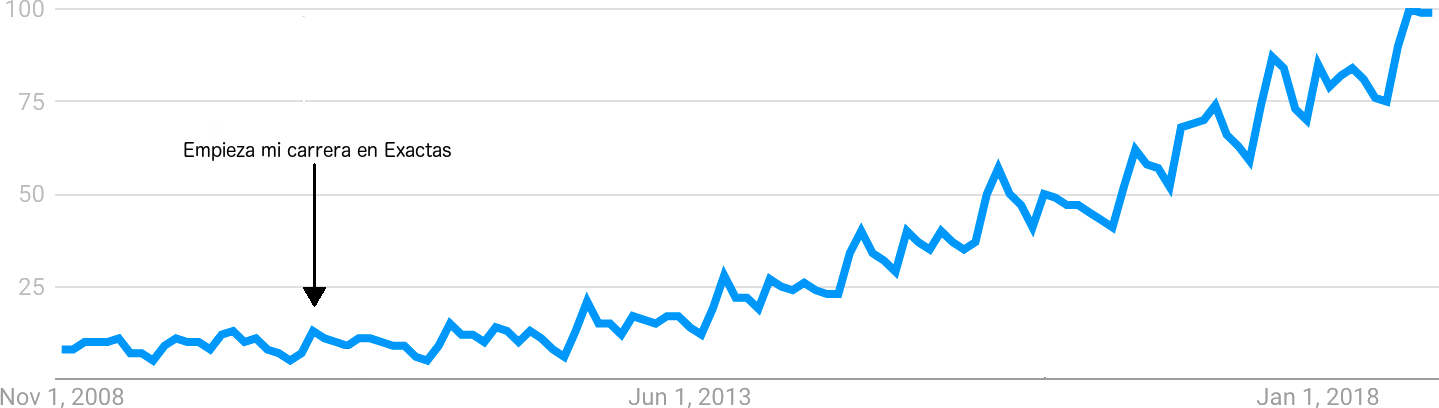
\includegraphics[width=\framewidth]{data_science_google_trends.png}
		\caption{Google trends for the term ``Data Science''\footcite{datasciencegt}}
	\end{figure}
	
\note{%
	En los últimos años hubo un crecimiento exponencial en la capacidad de acumular, guardar, y manipular cantidades masivas de datos sobre un gran espectro de disciplinas.

	Este crecimiento creó una pequeña revolución en muchas disciplinas académicas donde se solían usar encuestas u otros datos más particulares.
}
\end{frame}

\section{Marco Teórico}

\subsection{Homofília Social}

\begin{frame}
	\epigraph{``La gente ama a los que son como sí mismos.''}{\textit{Aristoteles \\ Retórica}}
	\note{%
		La similaridad lleva a la conexión.

		La gente tiene características, como edad, género, o estatus socioeconómico, con el que hay una mayor tasa de contacto que gente disimilar.

		El trabajo hecho en esta tesis está relacionado a descubrir y explotar casos de homofília en la población de un grafo social.
	}
\end{frame}

\begin{frame}
	\begin{figure}
		\begin{subfigure}[b]{0.48\framewidth}
			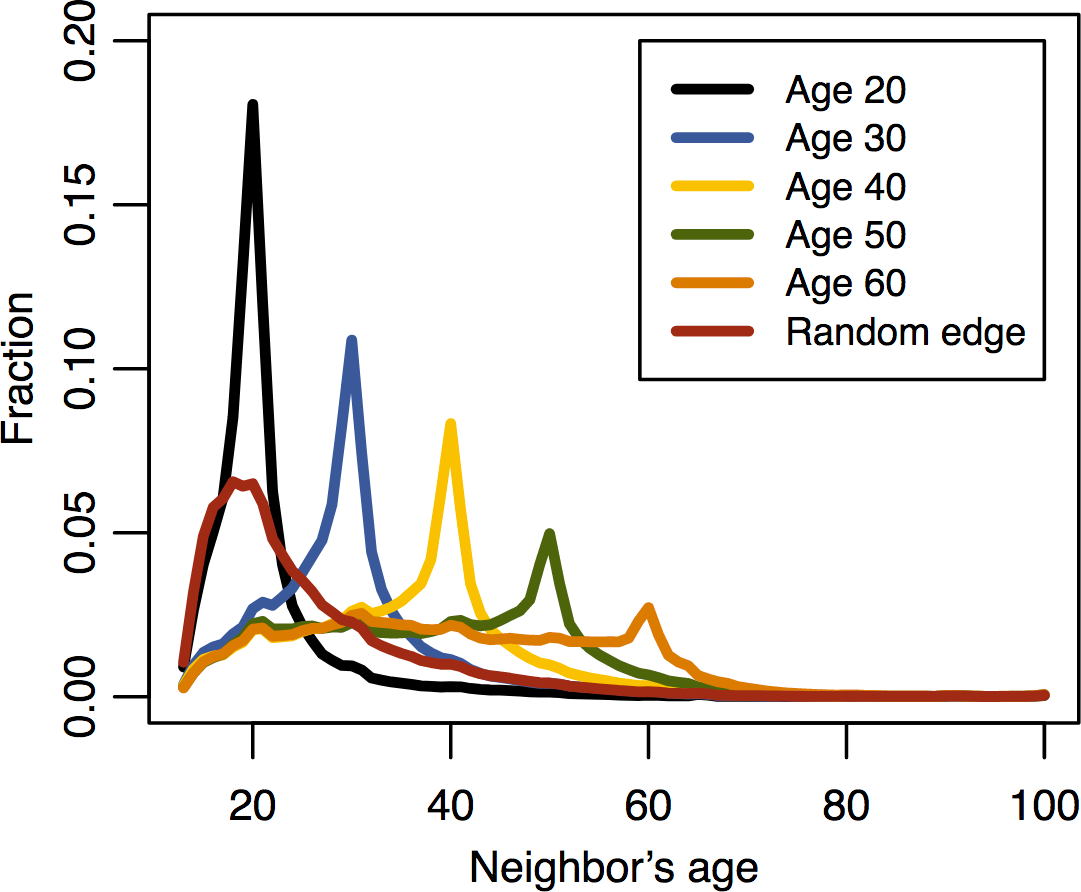
\includegraphics[width=0.9\textwidth]{age_homophily.png}
			\caption{}%
			\label{fig:age_homophily}
		\end{subfigure}
		\begin{subfigure}[b]{0.48\framewidth}
			\hfill{}
			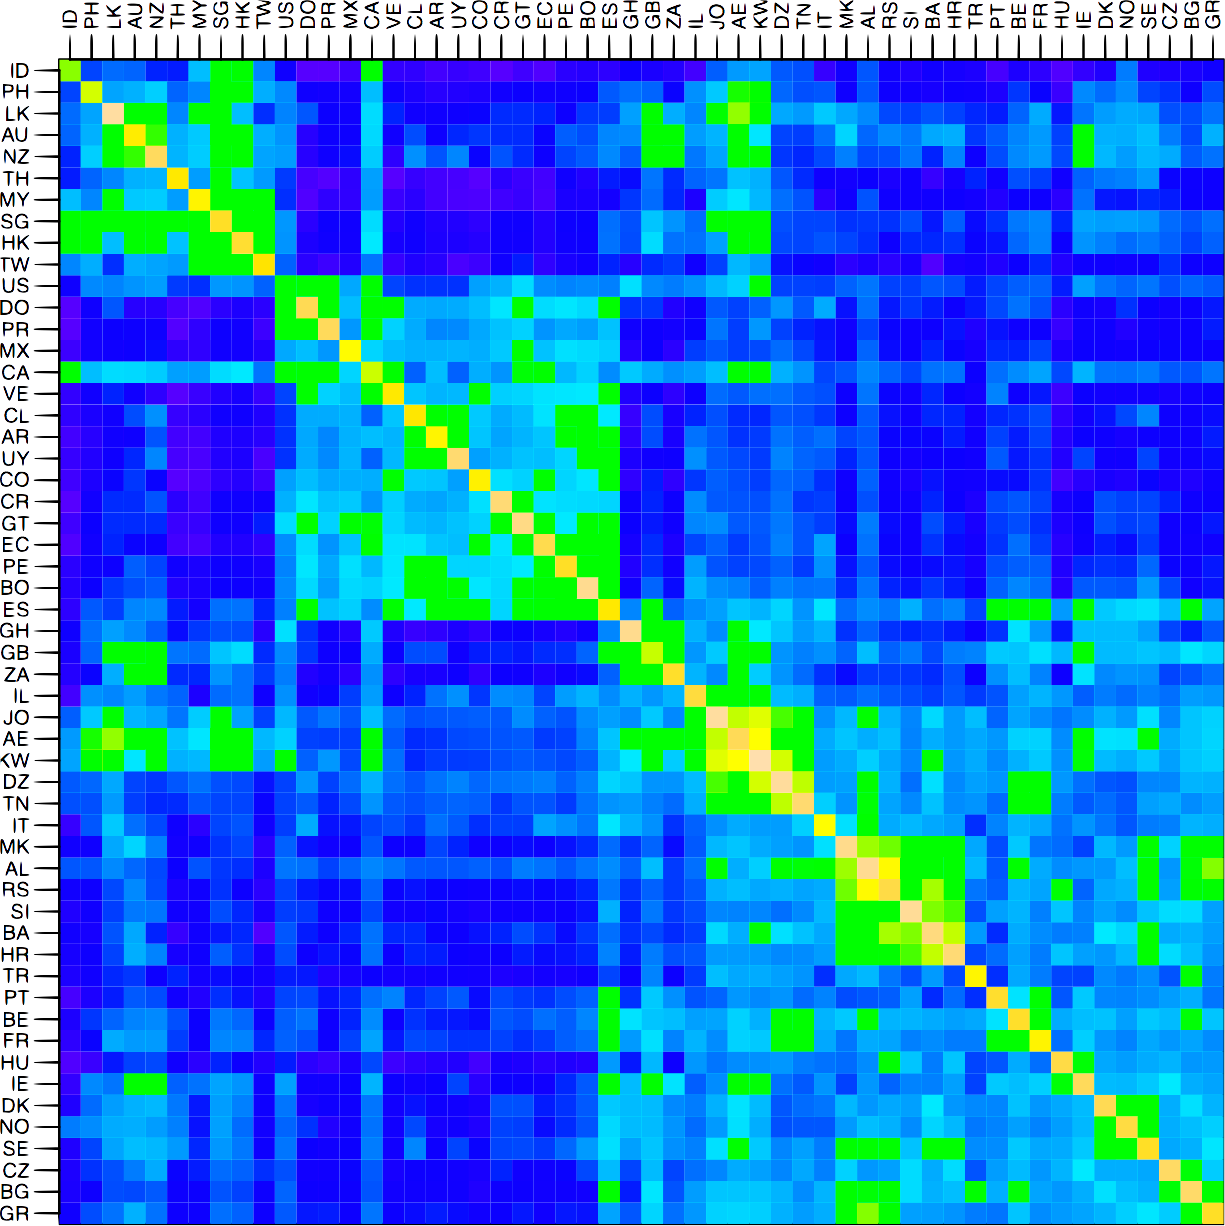
\includegraphics[width=0.9\textwidth]{country_homophily.png}
			\caption{}%
			\label{fig:country_homophily}
		\end{subfigure}
		\caption{Ejemplos varios de homofília en un cierto grafo social\footcite{ugander2011anatomy}. \subref{fig:age_homophily}: Distribución de edades para contactos de usuarios de cada edad. \subref{fig:country_homophily}: Mapa de calor marcando la cantidad normalizada de contactos entre cada par de países.}
	\end{figure}

	\note{%
		Dos casos muy comunes de homofília en grados sociales son la homofília por edad y la homofília por país. Ambas fueron investigadas por Ugander~et~al en el paper citado en este slide.

		Como se pueden apreciar en estos gráficos, el rango de edades para las conexiones de amistad en una red social están altamente sesgadas hacia la misma edad que tiene cada persona. También se puede ver lo mismo cuando se grafica los pares entre países entre todas las conexiones de amistad.
	}
\end{frame}

\subsection{Inferencia Bayesiana}

\begin{frame}{Inferencia Bayesiana}
	\parbox{.5\textwidth}{\raggedleft{}
		\begin{equation*}
			P \left( H \mid E \right) = \frac{P \left( E \mid H \right) \cdot P \left( H \right)}{P \left( E \right)}
		\label{eq:bayes}
		\end{equation*}
	}
	\hfill
	\parbox{.45\textwidth}{\raggedright{}
	\epigraph{``Dada la cantidad de veces en el que un evento desconocido sucedió y falló en suceder, la probabilidad de este pasando en una sola prueba está entre dos grados de probabilidad que pueden ser nombrados''}{\textit{Thomas Bayes \\ An Essay towards solving a Problem in the Doctrine of Changes}}
	}

	\note{%
		Parte de este trabajo usa enfoque bayesiano a las estadísticas. A diferencia del común enfoque frecuentista, donde los parámetros están fijos y desconocidos y las hipótesis son ciertas o falsas, cualquier cosa desconocida se describe con una distribución de probabilidad que describe su incertidumbre.
	}
\end{frame}

\begin{frame}{Teorema de Bayes}
	\begin{align*}
		&P \left( H \mid E \right) = \frac{P \left( E \mid H \right) \cdot P \left( H \right)}{P \left( E \right)} &\text{\textbf{Teorema de Bayes}} \\
		\vspace{4em} \\
		\alt<1> {%
		&P \left( H \mid E \right) &\text{\textbf{Posterior Probability}} \\
		&P \left( E \mid H \right) &\text{\textbf{Likelihood}} \\
		&P \left( H \right) &\text{\textbf{Prior Probability}} \\
		&P \left( E \right) &\text{\textbf{Marginal Likelihood}}
		}{}
		\alt<2> {%
			&P \left( H \mid E \right) \propto P \left( E \mid H \right) \cdot P \left( H \right) &\text{\textbf{Posterior Proportionality}}
		}{}
	\end{align*}
	
	\note{%
		\alt<1>{%
			El teorema de Bayes describe la probabilidad de un evento en base a conocimiento a priori de las condiciones posiblemente relacionadas a este. Este tiene cuatro términos.
			\begin{itemize}
				\item \textbf{Posterior Probability}, que es la probabilidad condicional asignada después de que el evento se toma en cuenta. \\
				\item \textbf{Likelihood}, el grado de probabilidad de $E$ dado que $H$ es cierto. \\
				\item \textbf{Prior Probability}, las suposiciones hechas en el problema antes de los experimentos. \\
				\item \textbf{Marginal Likelihood}, la función de probabilidad donde algunos parámetros fueron marginalizados. Se usa como constante normalizante para que la \emph{Posterior Probability} integre a $1$, haciendo que sea una probabilidad válida.
			\end{itemize}
		}{}
		\alt<2>{%
			Estas ecuaciones son probabilidadeso continuas, que por definición deben integrar a $1$. Por esa razón, se suele usar la ecuación en este \textit{slide}, que define la proporcionalidad del \textit{posterior}.
		}{}
	}
\end{frame}

\begin{frame}{Distribución Beta}
	\begin{gather*}
		X \sim B \left( \alpha, \beta \right) \\
		\begin{aligned}
			f \left( x; \alpha, \beta \right) &= \frac{1}{B \left(\alpha, \beta \right)} \cdot x^{\alpha - 1} {\left( 1 - x \right)}^{\beta - 1} \\
			F \left( x; \alpha, \beta \right) &= \frac{1}{B \left(\alpha, \beta \right)} \cdot \int^x_0 {t^{\alpha - 1} {\left( 1 - t \right)}^{\beta - 1} dt} \\
			\vspace{1em} \\
			B \left( \alpha, \beta \right) &= \frac{\Gamma \left( \alpha + \beta \right)}{\Gamma \left( \alpha \right) \Gamma \left( \beta \right)}
		\end{aligned}
	\end{gather*}
\end{frame}

\section{Trabajos Relacionados}

\begin{frame}
	
\end{frame}

\section{Fuente de Datos}

\begin{frame}
	
\end{frame}

\section{El Modelo Bayesiano}

\begin{frame}
	
\end{frame}

\section{Modelos Comunes de Aprendizaje Automático}

\begin{frame}
	
\end{frame}

\section{Resultados Finales}

\begin{frame}
	
\end{frame}

\section{Referencias}

\section{Agradecimientos}

\begin{frame}
	
\end{frame}

\end{document}
